\documentclass[tikz,border=3mm]{standalone}
\usetikzlibrary{matrix,positioning,fit,backgrounds}
\begin{document}
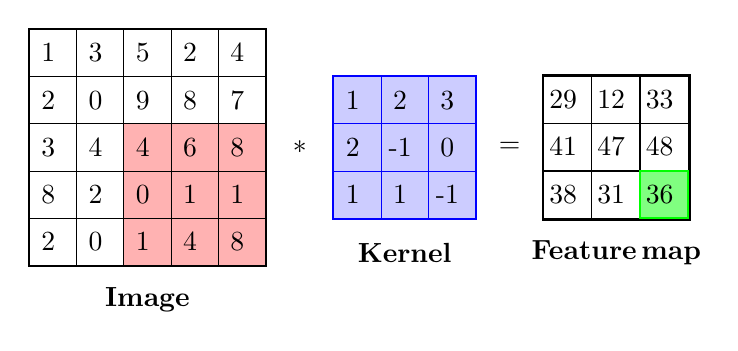
\begin{tikzpicture}[mmat/.style={matrix of nodes,
	column sep=-\pgflinewidth/2,
   row sep=-\pgflinewidth/2,
   cells={nodes={draw,inner sep=2pt,thin}},draw=#1,thick,inner sep=0pt},
  nodes in empty cells,
  nodes={
  	minimum size=.6cm,
  	anchor=center,
  	align=center,
  	},
   mmat/.default=black,
   node distance=0.3em]
 \matrix[mmat](mat1){
         1 & 3 & 5 & 2 & 4  \\ 
         2 & 0 & 9 & 8 & 7   \\ 
         3 & 4 & 4 & 6 & 8   \\ 
         8 & 2 & 0 & 1 & 1   \\ 
         2 & 0 & 1 & 4 & 8   \\ 
         };
 \node[right=of mat1] (mul) {$*$}; 
 \node [below= of mat1.south] (i) {$\bf Image$};
  
 \scoped[on background layer]
 {
 	\node[fill=red!30, fit=(mat1-3-3)(mat1-5-5),inner sep=0pt] {};
 }    
 \matrix[mmat=blue,fill=blue!20,right=of mul](mat2){    
     1 & 2 & 3 \\ 
     2 &-1 & 0 \\ 
     1 & 1 & -1 \\
 	};
 \node[right=of mat2] (eq) {$=$};
 \node [below= of mat2.south] (k) {$\bf Kernel$};
        
 \matrix[mmat, right=of eq](mat3){    
     29 & 12 &33 \\ 
      41 & 47  & 48 \\
      38 & 31 & |[draw=green, thick, fill=green!50]|36 \\ 
     };
 \node [below= of mat3.south] (f) {$\bf Feature\,map$};

 
\end{tikzpicture}
\end{document}
